% Copyright (c) 2026 CorrectBrain
% SPDX-License-Identifier: MIT

\PassOptionsToPackage{dvipsnames,svgnames,x11names}{xcolor}
\documentclass[tikz,border=8pt]{standalone}
\usetikzlibrary{arrows.meta,positioning,calc,shapes,shadows,decorations.pathmorphing,shapes.geometric,backgrounds,decorations.markings,decorations.pathreplacing,decorations.text,fit,shapes.misc,shapes.arrows,matrix,bending,3d,chains,intersections,shapes.symbols,svg.path,shapes.multipart,snakes,shapes.callouts,angles,quotes}
\providecolor{gold}{RGB}{212,175,55}
\providecolor{silver}{RGB}{192,192,192}
\providecolor{bronze}{RGB}{205,127,50}
\providecolor{darkblue}{RGB}{0,0,139}
\providecolor{lightblue}{RGB}{173,216,230}
\providecolor{darkgreen}{RGB}{0,100,0}
\providecolor{lightgreen}{RGB}{144,238,144}
\providecolor{darkred}{RGB}{139,0,0}
\providecolor{navy}{RGB}{0,0,128}
\providecolor{skyblue}{RGB}{135,206,235}
\providecolor{beige}{RGB}{245,245,220}
\providecolor{cream}{RGB}{255,253,208}
\usepackage{amsmath}
\usepackage{amssymb}
\usepackage{fontawesome5}
\usetikzlibrary{fadings,shadows.blur,patterns,patterns.meta}

\providecolor{gold}{RGB}{212,175,55}
\providecolor{silver}{RGB}{192,192,192}
\providecolor{bronze}{RGB}{205,127,50}
\providecolor{darkblue}{RGB}{0,0,139}
\providecolor{lightblue}{RGB}{173,216,230}
\providecolor{darkgreen}{RGB}{0,100,0}
\providecolor{lightgreen}{RGB}{144,238,144}
\providecolor{darkred}{RGB}{139,0,0}
\providecolor{navy}{RGB}{0,0,128}
\providecolor{skyblue}{RGB}{135,206,235}
\providecolor{beige}{RGB}{245,245,220}
\providecolor{cream}{RGB}{255,253,208}
\usepackage{amsmath}
\usepackage{amssymb}
\usepackage{fontawesome5}

% --- COLOR PALETTE ---
\definecolor{cssblue}{RGB}{41, 128, 185}
\definecolor{cssorange}{RGB}{230, 126, 34}
\definecolor{svgred}{RGB}{192, 57, 43}
\definecolor{darkgray}{RGB}{52, 73, 94}
\definecolor{lightbg}{RGB}{250, 252, 255}

\begin{document}
\begin{tikzpicture}[
    x=1cm, y=1cm,
    % --- STYLES ---
    infopanel/.style={
        draw=darkgray!30, fill=white, rounded corners=4pt,
        text width=5.5cm, align=left, inner sep=8pt, font=\footnotesize, text=darkgray,
        blur shadow={shadow opacity=15, shadow yshift=-1pt}
    },
    cssbox/.style={
        draw=cssblue, thick, fill=cssblue!5, dashed, rounded corners=2pt
    },
    svgbox/.style={
        draw=svgred, very thick, fill=svgred!10
    }
]

% Background (Pure White Rule)
\fill[white] (-15, 13.5) rectangle (22,-4.7136);

% --- 1. TITLE BLOCK ---
\node[fill=darkgray, text=white, rounded corners=6pt, text width=24cm, inner sep=12pt, align=center, drop shadow={opacity=0.3, shadow yshift=-2pt}] at (3.2952,12.261) {
    {\Large\bfseries \faIcon{expand-arrows-alt} \quad The CSS Bounding Engine \& Responsive Translation}\\[4pt]
    \normalsize How the extracted \texttt{viewBox="0 0 100 100"} dynamically conforms to flexible DOM containers.
};


% --- 2. SOURCE SVG (Left Side) ---
% Labels placed outside bounding box
\node[font=\bfseries\color{svgred}] at (-9,9.8336) {Source SVG viewBox};
\node[font=\footnotesize\color{svgred}] at (-9,9.3336) {(100 x 100 Abstract Units)};

% Bounding box (6x6 units)
\draw[svgbox] (-12, 3) rectangle (-6, 9);

% Internal 100x100 Mathematical Coordinate Grid
\draw[svgred!20, thin, step=0.6] (-12, 3) grid (-6, 9);

% Absolute Axis Coordinate Labels (Complete Mathematical Closure)
\node[font=\tiny\ttfamily, color=svgred!80, anchor=south east] at (-12, 9) {(0,0)};
\node[font=\tiny\ttfamily, color=svgred!80, anchor=south west] at (-6, 9) {(100,0)};
\node[font=\tiny\ttfamily, color=svgred!80, anchor=north east] at (-12, 3) {(0,100)};
\node[font=\tiny\ttfamily, color=svgred!80, anchor=north west] at (-6, 3) {(100,100)};

% Realistic Dimensional Vector Artwork (Scaled to center (-9, 6))
\shade[ball color=svgred!70, opacity=0.9] (-10.5, 7.5) circle (1);
\fill[svgred!80, drop shadow={opacity=0.3}] (-8, 4) -- (-6.5, 5.5) -- (-6.5, 4) -- cycle;
\draw[svgred, ultra thick, drop shadow={opacity=0.3}] (-11.5, 4) to[out=45, in=180] (-9, 5);


% --- 3. THE MAPPING ENGINE (Center) ---
\draw[fill=gray!5, draw=darkgray, thick, rounded corners=6pt, blur shadow={shadow opacity=15, shadow yshift=-1pt}] (-3, 4.5) rectangle (3, 7.5);
\node[font=\Huge\color{darkgray}] at (0, 6.7) {\faCogs};
\node[font=\bfseries\color{darkgray}, align=center, text width=5cm] at (0, 5.4) {CSS scaling \&\\ \texttt{preserveAspectRatio}\\ \texttt{="xMidYMid meet"}};


% --- 4. CSS SCENARIO A: WIDE DESKTOP CONTAINER (Top Right) ---
% Labels in safe zone above box
\node[font=\bfseries\color{cssblue}] at (10, 10.2) {Scenario A: Wide CSS Container};
\node[font=\footnotesize\ttfamily\color{cssblue}] at (10, 9.7) {width: 100\%; height: 250px;};

% CSS Container (8x4 units)
\draw[cssbox] (6, 5) rectangle (14, 9);

% Letterboxing zones with transparent checkerboard pattern (Horizontal)
\fill[pattern=checkerboard, pattern color=black!5] (6, 5) rectangle (8, 9);
\fill[pattern=checkerboard, pattern color=black!5] (12, 5) rectangle (14, 9);

% SVG placed inside (Scaled to 4x4, centered)
\begin{scope}[shift={(8, 9)}, scale=0.66667]
    \draw[svgbox, solid] (0, 0) rectangle (6, -6);
    \draw[svgred!20, thin, step=0.6] (0, 0) grid (6, -6);
    \shade[ball color=svgred!70, opacity=0.9] (1.5, -1.5) circle (1);
    \fill[svgred!80, drop shadow={opacity=0.3}] (4, -5) -- (5.5, -3.5) -- (5.5, -5) -- cycle;
    \draw[svgred, ultra thick, drop shadow={opacity=0.3}] (0.5, -5) to[out=45, in=180] (3, -4);
\end{scope}

% High-readability empty DOM space tags
\node[fill=white, draw=darkgray!20, rounded corners=3pt, inner sep=3pt, font=\scriptsize, align=center, text=darkgray] at (7, 7) {Empty\\DOM\\Space};
\node[fill=white, draw=darkgray!20, rounded corners=3pt, inner sep=3pt, font=\scriptsize, align=center, text=darkgray] at (13, 7) {Empty\\DOM\\Space};


% --- 5. CSS SCENARIO B: NARROW MOBILE CARD (Bottom Right) ---
% Labels in safe zone above box
\node[font=\bfseries\color{cssblue}] at (10,3.9455) {Scenario B: Mobile Card};
\node[font=\footnotesize\ttfamily\color{cssblue}] at (10,3.4455) {width: 50vw; height: 80vh;};

% CSS Container (4x7 units)
\draw[cssbox] (8, -4) rectangle (12, 3);

% Symmetrical Letterboxing Zones (Vertical)
\fill[pattern=checkerboard, pattern color=black!5] (8, 1.5) rectangle (12, 3);
\fill[pattern=checkerboard, pattern color=black!5] (8, -4) rectangle (12, -2.5);

% SVG placed inside (Scaled to 4x4, centered)
\begin{scope}[shift={(8, 1.5)}, scale=0.66667]
    \draw[svgbox, solid] (0, 0) rectangle (6, -6);
    \draw[svgred!20, thin, step=0.6] (0, 0) grid (6, -6);
    \shade[ball color=svgred!70, opacity=0.9] (1.5, -1.5) circle (1);
    \fill[svgred!80, drop shadow={opacity=0.3}] (4, -5) -- (5.5, -3.5) -- (5.5, -5) -- cycle;
    \draw[svgred, ultra thick, drop shadow={opacity=0.3}] (0.5, -5) to[out=45, in=180] (3, -4);
\end{scope}

% High-readability empty DOM space tags
\node[fill=white, draw=darkgray!20, rounded corners=3pt, inner sep=2pt, font=\scriptsize, align=center, text=darkgray] at (10, 2.25) {Empty DOM Space};
\node[fill=white, draw=darkgray!20, rounded corners=3pt, inner sep=2pt, font=\scriptsize, align=center, text=darkgray] at (10, -3.25) {Empty DOM Space};


% --- 6. PROCESS ROUTING & EXPLANATORY ANNOTATIONS ---
% Process Routing Arrows
\draw[-Stealth, ultra thick, darkgray!60] (-5.8, 6) -- (-3.2, 6);
\draw[-Stealth, ultra thick, darkgray!60] (3.2, 6.5) to[out=0, in=180] (5.8, 7);
\draw[-Stealth, ultra thick, darkgray!60] (3.2, 5.5) to[out=0, in=180] (7.8, -0.5);

% Info panel 1 (Fluid Variables)
\node[infopanel, text width=5.5cm] (info1) at (-9, -1.5) {
    \textbf{\color{svgred}\faIcon{draw-polygon} \quad Fluid Fractional Variables}\\[2pt]
    Inside the SVG, lengths are relative to the \texttt{100x100} abstraction. A circle with \texttt{r="25"} takes up 50\% of the \texttt{viewBox}, regardless of the actual CSS pixel size on the screen.
};
\draw[-Stealth, dashed, svgred, thick] (info1.north) -- (-9, 2.8);

% Info panel 2 ("Meet" Scaling Logic)
\node[infopanel, text width=5.5cm] (info2) at (17, -1.5) {
    \textbf{\color{cssblue}\faIcon{arrows-alt} \quad "Meet" Scaling Logic}\\[2pt]
    The default behavior (\texttt{xMidYMid meet}) scales the \texttt{viewBox} up or down until it hits the \textit{first} constraint of the CSS bounding box (either width or height). It then centers the graphic, maintaining the perfect 1:1 intrinsic ratio, leaving whitespace in the remaining dimension (Letterboxing).
};
\draw[-Stealth, dashed, cssblue, thick] (info2.west) -- (12, -1.5);

\end{tikzpicture}
\end{document}
